\exercise[Robot Control]

% forward rotatio

\subsection{3.1 Forward Kinematics}

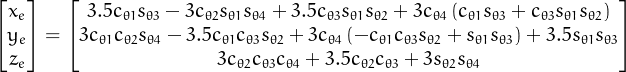
\includegraphics[]{x_y_z.png} \\

The accuracy using forward kinematics is way better than the one using vision. This is because forward kinematics uses the exact joint angles, and by construction, calculates the correct end effector position given the correct joint angles. Our vision part in contrast estimates the angles based on 3D location, which is constructed by using projects onto the yz and xz plane. As our robot end effector moves further from those planes, our vision estimates get less accurate.
\begin{center}
\begin{tabular}{|c|c|c|}
\hline
$(\theta_1 , \theta_2 , \theta_3, \theta_4)$ & Camera (x,y,z) & Forward Kinematics (x, y, z) \\\hline
 (0.3, 0.3, 0.3, 0.3) & (3.25, -2.66, 9.03) & (2.58, -1.97, 8.05) \\ \hline
 (-0.6, -0.6, 0.6, 0.6) & (4.26, -1.22, 8.92) & (3.57, -0.76, 7.53) \\ \hline
 (1.0, -0.6, 0.6, -1.0) & (-2.05, 5.29, 4.88) & (-2.2, 4.85, 4.56) \\ \hline
 (1.0, 0.6, -0.6, -1.0) & (-1.86, -3.02, 8.66) & (-1.31, -2.59, 7.41) \\ \hline
 (-0.5, 0.3, 0.1, -0.4) & (0.207, -1.09, 9.87) & (0.206, -0.94, 8.80) \\ \hline
 (-0.2, -0.2, -0.2, 0.7) & (-1.57, -0.69, 9.38) & (-1.28, -0.52, 8.45) \\ \hline
 (0.8, 0.8, 0.8, 0.8) & (7.27, -0.24, 3.23) & (5.87, -0.11, 3.67) \\ \hline
 (0.4, -0.3, 0.4, 0.2) & (1.86, 2.71, 9.01) & (1.84, 2.07, 8.43) \\ \hline
 (0.1, -0.1, 0.1, -0.1) & (0.60, 1.32, 9.95) & (0.55, 1.00, 8.89) \\ \hline
 (0.6, 0.5, -0.5, 0.5) & (-0.26, -4.83, 6.53) & (-0.45, -6.07, 7.63) \\ \hline
\end{tabular}
\end{center}
\subsection{3.2 Closed-loop control}
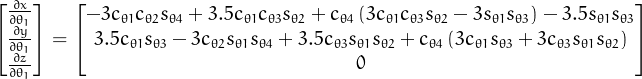
\includegraphics[]{jac_col1.png} \\ \\
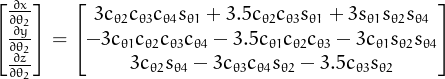
\includegraphics[]{jac_col2.png} \\ \\
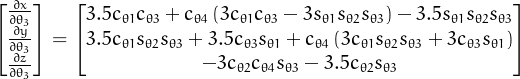
\includegraphics[]{jac_col3.png} \\ \\
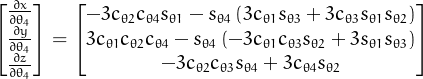
\includegraphics[]{jac_col4.png} \\
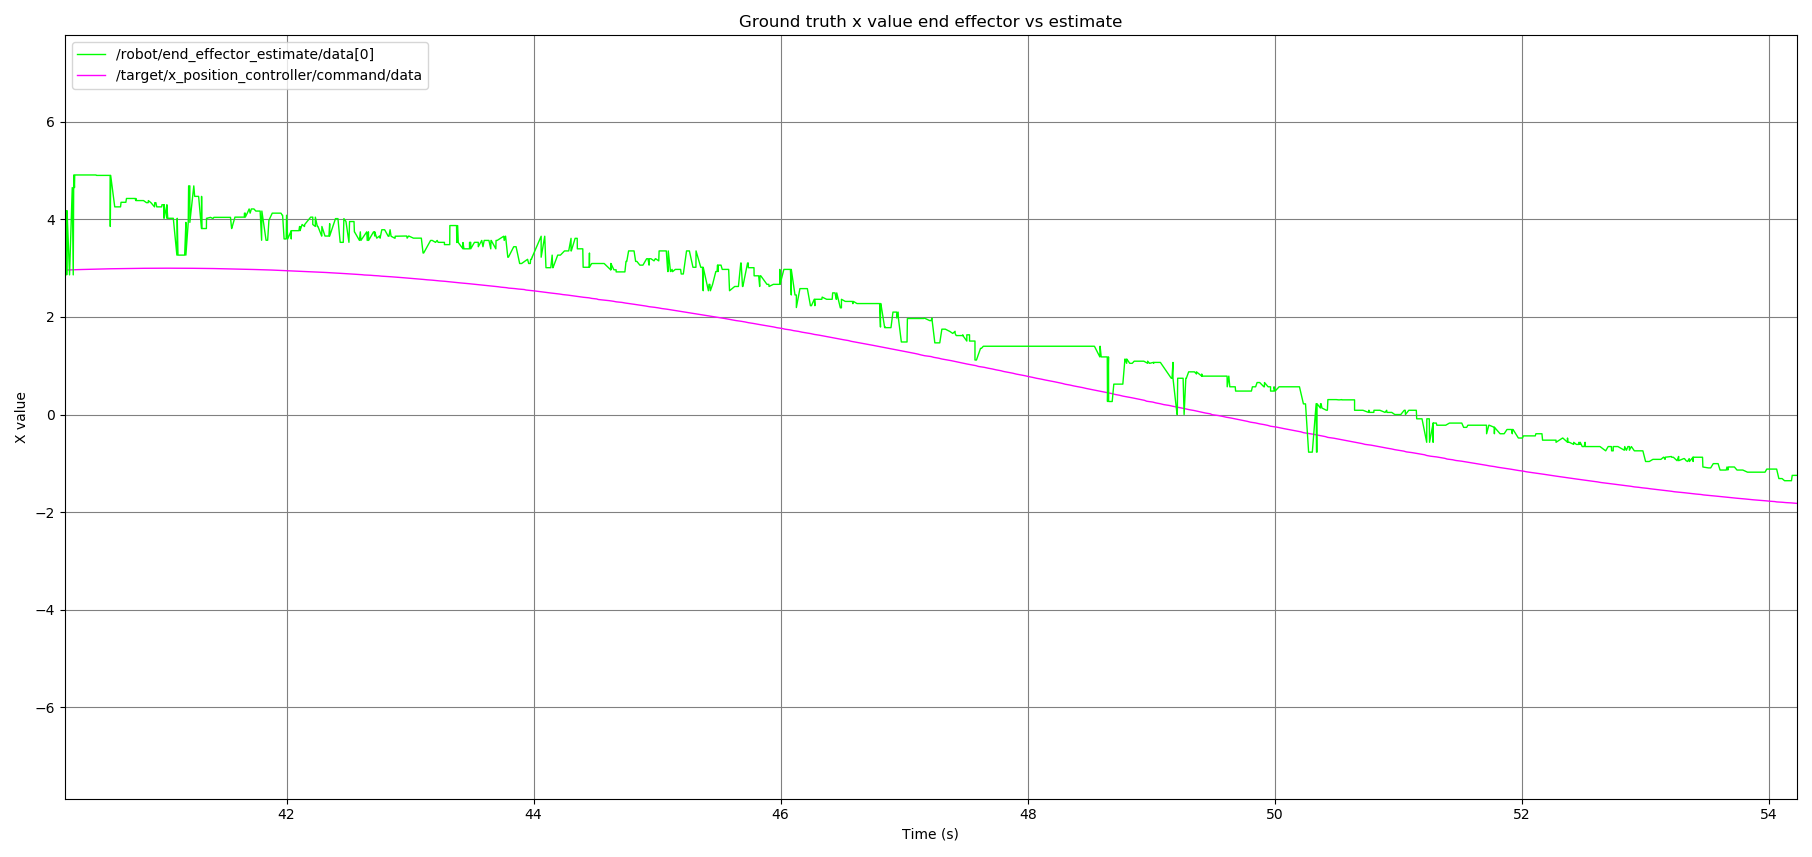
\includegraphics[width=0.9\textwidth]{plots/closed_x.png} \\
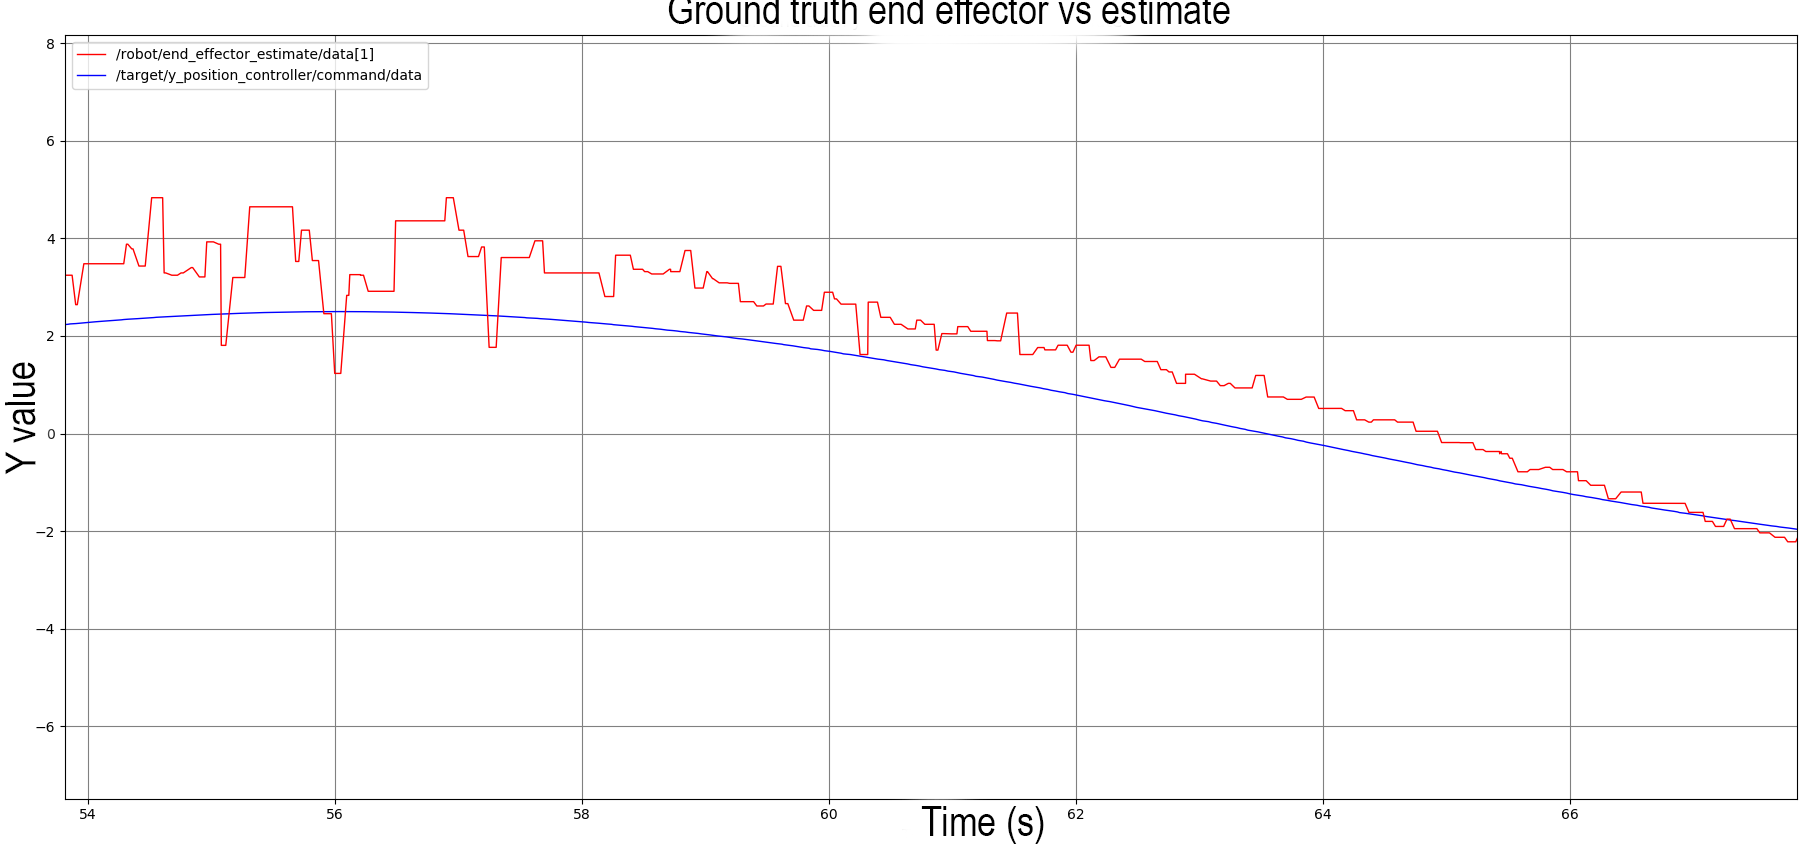
\includegraphics[width=0.9\textwidth]{plots/closed_y.png} \\
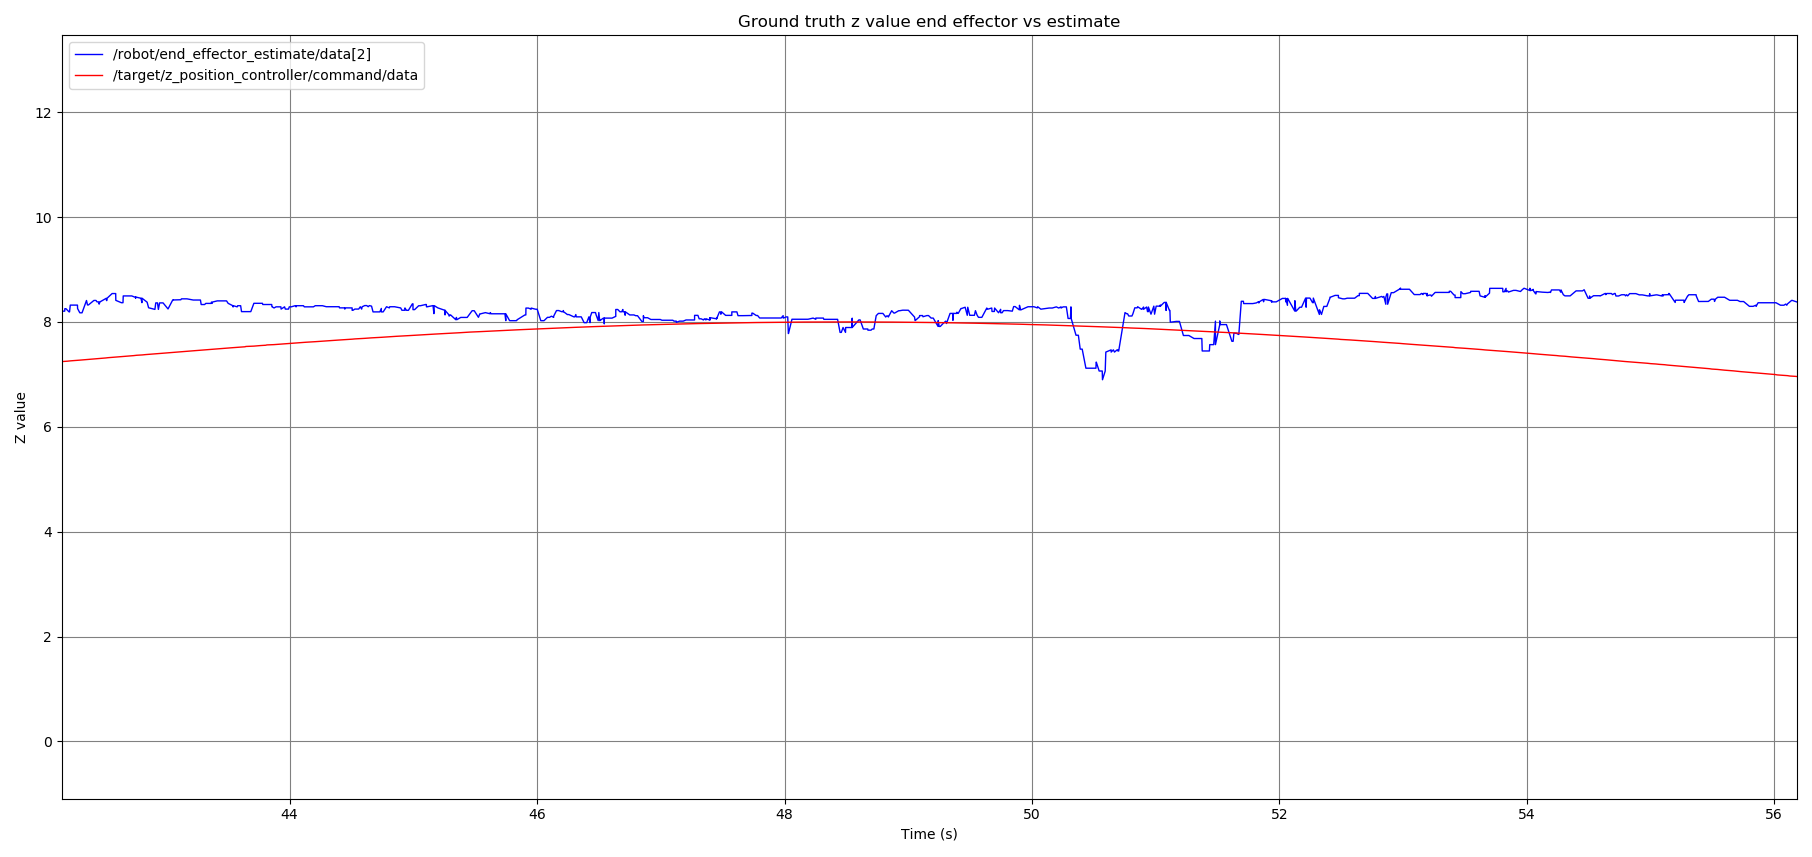
\includegraphics[width=0.9\textwidth]{plots/closed_z.png}
